\section{Programming Security}

\begin{definition}[Accessory controls]
	If a company X notices that a part P of a product does not belong to them,
	they may reduce the effectiveness of the product.

	For example, if a printer notices a competitors ink in the printer, it 
	may go from high quality to low.

	This is considered a form of authentication.
\end{definition}

\begin{definition}[Access control]
	I assume the meaning is intuitive to understand.
	What's worth mentioning is that access control can operate on four levels,
	namely:
	\begin{itemize}
		\item Application
		\item Middleware
		\item Operating system
		\item Hardware
	\end{itemize}
\end{definition}

\begin{definition}[Access Control Lists]\label{ACL}
	Most UNIX-fans will know them already: 
		\textit{-rw-r--r-- 1 $<$owner of file$>$ $<$group owner of file$>$.}
	This is an example of a rowwise mandatory ACL- where an object
	has a given set of definitions for three different groups:
	the first three letters in the string denotes what the owner can do
	(in this case, there is no execution, but read and write),
	the third next letters (mid-block) denote what members of the
	owner group can do to the file, and the next three letters denote
	what everyone else can do.

	This type of ACL are slow for systems with many users. 
	The vantage is that is efficient. Other forms of ACL's include
	database access control (suffering from inability to model
	states, etc.
\end{definition}
\begin{minipage}{\linewidth}
\makebox[\linewidth]{% center the image
  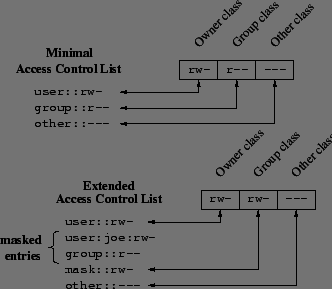
\includegraphics[keepaspectratio=true,scale=0.6]{./ACLnix.png}}
  \captionof{figure}{Typical UNIX ACL}% only if needed
  \label{visina8}

\end{minipage}

\begin{definition}[Assurance classes]
\end{definition}

\begin{definition}[Authentication]
	To prove that you are who you claim to be. E.g.\ to provide a password
	for an account, etc.
\end{definition}

\begin{definition}[Authorization]

	To ensure that a user has sufficient permissions to do what he/she
	asks for. E.g.\ an authenticated user may log in, but may not
	change the passwords for other users, because this authenticated user
	is not authorized for this account.
\end{definition}

\begin{definition}[BAN-logic]
	IS THIS REALLY NECESSARY?

	\dots formal reasoning in cryptology, somewhat alike first-order-logic.
\end{definition}

\begin{definition}[Biba Model]\label{biba}
	Essentially BLP, just that it is read by "no read down, no write up".
	The BLP can be categorized as "no write down, no read up".

	\epigraph{A monk may write a prayer book that can be read by commoners, 
	but not one to be read by a high priest}
	{--- \textup{Wikipedia}}

\end{definition}

\begin{definition}[Bell LaPadula model]
	Any system that adheres to the two following properties, are said to
	adhere to the Bell LaPadula Model, which is a \nameref{secpol}:
	\begin{description}[labelindent=1cm]
		\item[Simple security property] 
			\textit{no process may read data at a higher level.}
			If a process is on runlevel X, it should not have access to data at level 
			X + 1.
		\item[*-property]
			\textit{no process may write data to a lower level.} Imagine 
			that a sysadmin gets a Trojan that reads much sensitive data. 
			The *-property prevents this data to be written down to a lower level
			where it is accessible to other accounts with lower clearance.
	\end{description}

	It is worthwile noting that the properties fail to mention policies
	for creation and destruction of files.
	Furthermore, the model is broken if sensitive data is temporarily declassified. 
	The data can then be manipulated without violating the constraints of BLP.\
	Hence, to make the BLP safe, we need to introduce the 
    \textbf{tranquility property}:
	\begin{description}[labelindent=1cm]
		\item[Strong:] 
			Security labels on objects never change during systems operation.
		\item[Weak:]
			Security labels never change in such a way that it defines the
			given security policy.
	\end{description}

	However, the problem with the tranquility property is that process will 
	have a difficult time reading files. If at first one reads something at 
	a high level, then no concurrent read/write operation can occur for a lower
	level. Applications will therefore need to be customized extensively to accomodate
	for the tranquility property.

	The BLP only deals with confidentiality, not integrity (see~\nameref{biba})
\end{definition}

\begin{definition}[Biba Model]
	Deals with integrity alone, ignores confidentiality.
\end{definition}

\begin{definition}[BMA model]
	British Medical Association. 
	Basically a 9-point long list wich comprehends the BLP,
	but also represents state, and so on. Used for medical records.

	It's worthwhile noting that for medical records, it's much harder to
	define privacy and such because doctors are often required to involve
	third parties with their records. This could be researchers, drug companies,
	family, so on.
\end{definition}

\begin{definition}[Capture error]
	People are used to clicking "OK" on alert boxes without reading, so you
	might fool them intro clicking on one of your buttons by simply 
	making a popup box.
\end{definition}


\begin{definition}[Chinese Wall]
	Lets say that you work in finance, reviewing different oil companies.
	If you've worked on account A for some time, you might have information
	that is relevant for account B. To prohibit this, you're given
	a timed restriction, such that you cannot work on other accounts 
	if you have sensitive information.

	The general idea is to say that "you can access this, but nothing else,
	there's a chinese wall between you and other accounts."

	The chinese wall has been expressed to be similar to the BLP.\
	Let $c$ denote objects of interest, for example bank data. $s$ 
	denotes a subject, for example a person, who tries to access objects.
	$y(x)$ is a function $y$ for an object $x$ that denotes a company $y$'s 
	interest for the object $x$. Similarily, for a company $f$, there's a 
	function $f(x)$. The domain $S = S(s)$ is a set which covers all
	objects that $s$ can access.

	\begin{description}[labelindent=1cm]
		\item[Simple security property]
			$\forall s$, $s$ will have access to $c$ iff $\forall o \in S(s)$
			, $y(c) \cap x(o) = \emptyset$ or $y(c) \in y(o)$
		\item[The *-property]
			$s$ can write to an object $c$ iff $\forall o\{m \| m \in S(s) \} ),
			o \notin x(c) $ and $y(c) \neq y(o)^{[what?]}$
	\end{description}
\end{definition}

\begin{definition}[Common Criteria]\label{cc}
	Defines many~\nameref{secfunreq}. ISO-standard.
\end{definition}

\begin{definition}[Confidentiality]
	\textit{Who/what could have read this message?}
\end{definition}

\begin{definition}[Covert channel]
	If a system adheres to the BLP, a low security object might still
	commuicate with one at a higher level. If the two share a resource,
	e.g.\ a disc, one could make the higher level process do something
	with the disc head to communicate. This could for example be invoking 
	an error at time $t_{i}$ to indicate that bit $i$ in an important file is
	either 1 or 0. This way of communication is called a covert channel.
\end{definition}


\begin{definition}[Cryptographic nonce]\label{nonce}
	a nonce is an arbitrary number used only once in a cryptographic communication.
	The nonce is there to ensure freshness of a message, e.g.\ it could be a
	timestamp. That way, one can be assured that encrypted messages are
	recent and not old.
\end{definition}

\begin{definition}[CSRF]
	performs an action on the server. The user is typically not aware 
	of what he/she is doing. I.e., if there is a URL that can be used
	to purchase 50 cars, Eve can send that to Alice and make her, unwillingly,
	buy 50 cars.

	CSRF attack can be mitigated by properly implementing session authentication
	tokens, such that one cannot modify/use an account without having a 
	valid token from the server. That way, the POST to purchase cannot be
	instantiated unless the client performs a series of steps.
	$\qedhere$
\end{definition}

\begin{definition}[Discretionary Access Control]\label{DAC}
	A simple form of access control. The ease of implementing DAC makes it popular.
	DAC is similar to~\nameref{mac}, except
	from that there are no \textit{policies} for objects. This means that
	whenever a subject wants to apply an action to an object $o$,
	the operating system will only evaluate $s$ and $o$, not the action that $s$ wants 
	to apply, in order to determine whether or not $s$'s action will be executed.
\end{definition}

\begin{definition}[Difference between DAC and MAC]\label{diffDACMAC}
	DAC is not a multilevel security protocol in that, for any subject 
	$s$, \textbf{any} operation on an object $o$ is either granted or not 
	\textbf{only by considering the relationship between $s$ and $o$, not
	the action applied}.
	
	Furtherly, the following quotes quite sum it up:
		\epigraph{Systems can be said to implement both MAC and DAC simultaneously,
		where DAC refers to one category of access controls that subjects can 
		transfer among each other, and MAC refers to a second category of access 
		controls that imposes constraints upon the first.}{--- \textup{Wikipedia}}

		\epigraph{In general, when systems enforce a security policy independetly 
		of user actions, they are described as having madatory access control,
		as opposed to the discretionary access control in systems like Unix where 
		users can take their own access decision about their files}
		{--- \textup{Page 246 in the book}}
\end{definition}

\begin{definition}[Evaluation Assurance Level]
The~\nameref{cc} uses 
\end{definition}

\begin{definition}[Format string vulnerability]
	Input data will be used to format output. However, the input data
	goes to the stack, and there are therefore vulnerabilities.
\end{definition}

\begin{definition}[High water mark principle]
	Start off at the bottom and elevate permissions as you need them.
	E.g.\` as one opens a mail client, one finds 
\end{definition}

\begin{definition}[Identify Friend or Foe]{IFF:}\label{iff}
	A system that can tell whether you are a friend of a foe.
	A classical crypto-problem; how can I know that I am not talking to Eve?
\end{definition}

\begin{definition}[Integer manipulation attack]
	Causing an under- or overflow or truncation such that you can 
	exploit software.
\end{definition}

\begin{definition}[Integrity]
	\textit{Who/what could have altered this package?}
\end{definition}

\begin{definition}[Kernel bloat]
	E.g.\ in Windows, you need to have many drivers run as root in the kernel.
	This will naturally open up for more security holes. 
\end{definition}

\begin{definition}[Key-distribution]\label{keydistribution}
	One entity on a network wants to talk to another in a network. 
	We will assume Alice wants to talk to Bob.
	Her concern is that they might establish a connection,
	but Eve might hijack it and pretend to be either party. Alice needs to know
	that she is speaking with Bob, and she needs to know that Bob is not 
	communicating with any Eve.

	To prevent this, a trusted third party is introduced. We will call this Sam.
	We will assume that the connection to Sam is safe, and that Sam knows 
	every user of the network.
	Alice contacts Sam. Her request is as follows: "I am Alice, and want to 
	communicate with Bob". Sam returns two tokens. The first token 
	can only be read by Alice, and the second only by Bob. Alice then contacts 
	Bob, giving him only the second certificate. Bob decrypts the certificate,
	which unravels an encryption/decryption key. Bob and Alice can now 
	encrypt and decrypt messages to each other using this key, and communicate
	without Sam.

\end{definition}

\begin{definition}[Landing pad]
	A piece of code, such that when exectued, the processor
	will exectue malicious code.
\end{definition}

\begin{definition}[Lattice model]
    Essentially equivalent to the BLP.\ You use labels such as "TOP SECRET",
    "SECRET" and say that there are no communications between levels as in the
    BLP.\

    You combine things, so for each item, e.g.\ for "missiles" you might have a
    clearance for something like "SECRET". But you also need codewords, such as
    "SECRET MISSILES" if you want to read the
	secret stuff about missiles.

    The point of the lattice model is that you have aggregated values, such
    that a lattice will yield a numeric $d$. To get access to $d$ you need $e >
    d$.
\end{definition}

\begin{definition}[Malware]
\end{definition}

\begin{definition}[Mandatory Access Control]\label{mac}
	\textit{Also known as multilevel security}.
	MAC is enforced as follows: for each object $o$, define a set of 
	actions that are applicable to this object, and categorize them by access level. 
	E.g.\ one could define deletions as \textit{administrator-level} and modifications as 
	\textit{user-level}. The categorization of actions to objects is known as
    defining the \textbf{policy}. The policy is often stored as
    an~\nameref{ACL}.  Typical values for $o$ include files, directories,
    ports, etc.  When subject $s$ requests an action $a$ on $o$, the operating
    system looks up the rules for $o$, finds $a$, and evaluates $s$ against the
    policy for $a$ on $o$.

	To clarify: in MAC, there is no such thing as "super-user-access", i.e.\
	being a user with high privileges won't necessarily grant you privileges on all
	objects, because some objects might have policies that only permit certain
	other users to manipulate them. For example, even though you might
	be a system administrator, you should not be able to read other user's
	passwords, nor modify them. You might rather grant sysadmins the privilege
	to reset the password, and let authenticated users modify their own passwords.

	MAC ensures a security policy indepent of user actions. That is, 
	even though a user owns a file, he/she might not be able to do 
	whatever he/she wants with it.
	
	A good example of the usefulness of MAC is that a computer that is hacked
	may not jepordize other systems. Despite of having obtained some level
	of control, the attacker may not get access to other critical features.

	MLS's are usually difficult to implement. One example is the 
	\textbf{cascading} problem; two systems A and B may both have access to an object $o$.
	Simeltaneously, system A have access to another object $a$, system B
	has access to object $b$, where $ a \neq b$. Now, modifying $o$ might
	affect how $a, b$ are treated. So if system B wants to alter
	$a$, it may modify $o$, then system A reads $o$, then modifies $a$.

	Do also note figure~\ref{xkcdauth} as it highlights a security
	caveat of MLS; low-level data can also be worthwhile protecting.
	See also the quote in \nameref{diffDACMAC}
\end{definition}
\begin{minipage}{\linewidth}
\makebox[\linewidth]{% center the image
  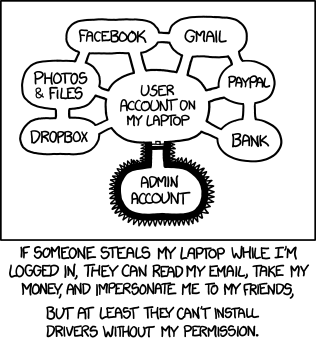
\includegraphics[keepaspectratio=true,scale=0.6]{./xkcd_auth.png}}
  \captionof{figure}{xkcd.com/1200}% only if needed
  \label{visina8}
\end{minipage}\label{xkcdauth}


\begin{definition}[No-operation]{NO-OP:}
	From assembly, do nothing. 
\end{definition}

\begin{definition}[Phishing]
	Essentially the same as~\nameref{pretext}ing, just that you're trying to
	decieve customers instead of staff.
\end{definition}

\begin{definition}[Pretext]\label{pretext}
	To create a plausible scenario that can decieve personell with 
	sensitive information to disclose this to Eve.
\end{definition}

\begin{definition}[Principle of least privilege]
	Programs should only have as much privilege as they need.
	There's no need to "sudo webbrowser"

\end{definition}

\begin{definition}[Protection profile]
	A document that identifies the desired security properties of a product.
	This is structured as a list of security requirements defined 
	in a way that adheres to~\nameref{cc}
\end{definition}

\begin{definition}[Pump]
	A one way transfer (data diode) that takes data from
	a low access level to a higher access level. 
\end{definition}

\begin{definition}[Race condition]
	Process A reads resource X, process B reads resource X,
	process A writes, then process B writes. The value is bad, since B's
	original value was bad.
\end{definition}

\begin{definition}[Reflection attacks]
	First, see~\nameref{chalres}.
	Suppose that the challenge-response is similar for two
	entities. I.e.\ party A sends a challenge $N$ to someone.
	To solve the challenge, party E simply returns $N$ to $A$,
	has party A solve it, and voila, party E knows the solution to $N$.
\end{definition}

\begin{definition}[Replay attack] 
	Assume that to login, Alice encrypts her password with one million bits
	, three times, and sends her password to a login page. The login
	decrypts and accepts Alice's authentication token.

	Eve could simply sniff the POST from Alice and the replay it to the 
	server. Even though the password is highly encrypted,
	Eve's POST will be valid. The login page accepts Eve.

    To mitigate, one should/could implement session tokens;
    see~\nameref{sessiontoken}. As mentioned in that section, however, session
    tokens also introduce other risks.
\end{definition}

\begin{definition}[Repudiation attack]
	To give someone a bad reputation. This could be by rating items
	with low scores, writing mean reviews, etc.
\end{definition}

\begin{definition}[Role based access control]
	Permissions are not related to users, but rather their functions. 
	This means that if a sysadmin is sick, a second-in-rank user could
	assume the rank of the sysadmin to do whatever is necessary.
\end{definition}

\begin{definition}[Sandbox]
	A limited environment. It is common to host websites in sandboxes,
	so that even if the webserver is hacked, a hacker can't do much on the
	mainframe.
\end{definition}


\begin{definition}[Security Policy (model)]\label{secpol}
\end{definition}



\begin{definition}[Secrecy]
\end{definition}

\begin{definition}[Security assurance requirements]

\end{definition}

\begin{definition}[Security functional requirements]\label{secfunreq}
	
\end{definition}

	\epigraph{A document that expresses clearly and consicely what the 
	protection mechanisms are to acheieve. \dots It will often take the form of 
	statements about which users may access which data}{--- page 240}

	As with most computer policies, it's important the statements
	are succint, i.e.\ briefly and clearly expressed, without implications. 
	Also, it's important to make sure that you explicitly define:
	\begin{itemize}
		\item Who determines the policy?
		\item What qualifies for "need to know"?
		\item How will the policy be enforced?
	\end{itemize}

\begin{definition}[Security requrement]
	A statement which defines what level of security is utilized
	for different kind of attacks.
	It's important that the requirements do not discuss design,
	only what is required (hence, requirement).

	All requirements should be testable. Good ways to do this is 
	to quantify. Quantifying security is difficult, however.
\end{definition}

\begin{definition}[Security target]
	A document that describes what a product does, 
	or at the very what it does that has an impact/relevance in security contexts.
\end{definition}

\begin{definition}[Session token]\label{sessiontoken}
	\textit{Also known as session ID or session identifier}. 
	A session token is a unique identifier, usually in the form of a hash
	generated by a hash function that is generated and sent from a server to a 
	client to identify the current interaction session.	
	
	If Eve can obtain the session ID, she can also, in theory, perform 
	actions, pretending to be the victim. This is known as \textbf{session hijacking}.
	As the session ID needs to be submitted for every POST and GET, it can
	be easy to obtain it by sniffing or tricking the victim. Hence, there
	should also be other security measures in place to make the use of session
	tokens safe.
\end{definition}


\begin{definition}[Smashing the stack]
	Making an overflow such that excess bytes are considered as code 
	rather than arguments.
\end{definition}

\begin{definition}[Software Security Touchpoints]
\end{definition}


\begin{definition}[SQL-injection]
	If you can't define this, please go get some sleep.
\end{definition}

\begin{definition}[Target of Evaluation]{ToE.}
	The product under evaluation.
\end{definition}

\begin{definition}[Trojan]
	A piece of software that looks cool, but in reality it causes harm
	when executed.
\end{definition}

\begin{definition}[Two-channel authentication]
    I fail to see the big differnece from~\nameref{twofactor}
	but accoding to the book, this is "sending an access code the user
	via a separate channel"
\end{definition}

\begin{definition}[Two-factor authentication]\label{twofactor}
	To authenticate, you need "something you have, and something you remember".
	E.g.\ a password and a password calculator.

	Most companies are sceptical of this. While it does seem to improve
	security per today's date, it is still prone to real-time mitm attacks.
\end{definition}


\begin{definition}[validation of input]\label{validation}
	Given input $\iota$, filter any bad input $b$ and return $\iota_{clean}$
	There are multiple types of input validation:
	\begin{description}[labelindent=1cm]
		\item[Blacklist-validation] do not regard context and trim away any bad 
			characters from input. 
			I.e.\ one can define a set of bad characters in a set
			$S = \{ ' , " , \ \}$, etc. Given input $\iota$, return 
			$\iota_{clean}$, s.t. $\iota_{clean} \cap S = \{\emptyset\}$
			The problem with black-validation is that is often easily bypassed,
			since the attacker can often distort his input in a way that bypasses
			the filters. Note that the filter only checks for characters, not context.
		\item[Whitelist-validation]
			In many contexts, the character ' is considered malicious, however,
			it is also required in some names, etc. White-validation looks
			at what structure input should have, and validates accordingly.
			It is stronger than blacklist-validation in that, for example 
			for dates it is possible to know what structure the input should have
			, and thereby you can trim from character length and structure.

			It is also worhtwile to talk of this as contextual encoding.
	\end{description}
	
	Another form of validation is the translation of characters to another typeset.
	This is typically known as \textbf{escaping} input. Before using any
	input one can e.g.\ do html-escaping. I assume the reader knows what this is.
	Character escaping has a recommended order: first do HTML-escaping, then
	JS-escaping. Finally, it is worth mentioning about escaping that it 
	does not prevent XSS, it just makes it harder to render data as code$^{[why?]}$.
\end{definition}

\begin{definition}[Valet attack]
	Assume that you use a random number in your key to unlock something, 
	like a car. This means that whenever you want to unlock the car, there
	are different codes, all valid. 
	
	If Eve gets to unlock Alice's car every day, Eve can record all keys used
	to unlock Alice's car. Eventually, when Alice's car run out of memory,
	it will not remember that the first key has ever been used. Eve
	then tries to use this first key that she recorded. This unlocks the car.
\end{definition}

\begin{definition}[Virus]
\end{definition}

\begin{definition}{XSS}
	upload a script that to a server that will be executed by other users.
	XSS is a popular type of attack and hence there's a lot of 
	terminology\dots
	\begin{description}[labelindent=1cm]
		\item[Stored XSS] the malicious script sent by an attacker is stored
			permanently on the webserver.
		\item[Reflected XSS] the malicious script sent by an attacker 
			causes an immediate malformed response from the server, but
			the script will not be stored on the server.
		\item[DOM-based XSS] typically sends a URL to a user such 
			that his/her site, i.e.\ DOM, is modified. E.g.\
			if the values for a selection field is specified from the url,
			modifying the parameters to be scripts instead
			means that the DOM is modified via XSS.
	\end{description}
	\epigraph{Reflected and Stored XSS are server side
	execution issues while DOM based XSS is a client (browser) side 
	execution issue}{--- \textup{OWASP}, https://www.owasp.org/index.php/DOM\_based\_XSS\_Prevention\_Cheat\_Sheet}
	

	Mitigations: see~\nameref{validation}
\end{definition}
